This means
\begin{equation}
	\begin{split}
		\mathbb{E}[C|D,I] &= \sum_{t=1}^{\infty}\gamma_{\text{disc}}^{t} \bigg[\frac{h_t+c_t}{\Gamma(N_0+\upsilon_t)}\bigg(
		\Gamma(N_0+\upsilon_t+1,\lambda_t)-\lambda_t\Gamma(N_0+\upsilon_t,\lambda_t)
		\bigg)\\
		&\qquad- c_t(N_0 + \upsilon_t-\lambda_t)\bigg]
	\end{split}
\end{equation}
Using
\begin{equation}
	\Gamma(N_0+\upsilon_t+1,\lambda_t) = (N_0+\upsilon_t)\Gamma(N_0+\upsilon_t,\lambda_t)+\lambda_t^{N_0+\upsilon_t}e^{-\lambda_t}
\end{equation}


\begin{equation}
	\Gamma(N_0+\upsilon_t+1,\lambda_t)-\lambda_t\Gamma(N_0+\upsilon_t,\lambda_t) = (N_0+\upsilon_t-\lambda_t)\Gamma(N_0+\upsilon_t,\lambda_t)+\lambda_t^{N_0+\upsilon_t}e^{-\lambda_t}
\end{equation}

\begin{equation}
	\begin{split}
		\mathbb{E}[C|D,I] &= \sum_{t=1}^{\infty}\gamma_{\text{disc}}^{t} \bigg[
		(h_t+c_t)(N_0+\upsilon_t-\lambda_t)\frac{\Gamma(N_0+\upsilon_t,\lambda_t)}{\Gamma(N_0+\upsilon_t)}+(h_t+c_t)\frac{\lambda_t^{N_0+\upsilon_t}e^{-\lambda_t}}{\Gamma(N_0+\upsilon_t)}\\
		&\qquad- c_t(N_0 + \upsilon_t-\lambda_t)\bigg]
	\end{split}
\end{equation}
To proceed, several approximations are invoked, starting with $N_0+\upsilon_t-\lambda_t \approx 0$ and Stirling's approximation of the gamma function
\begin{equation}
	\Gamma(N_0+\upsilon_t)\simeq \sqrt{2\pi (N_0+\upsilon_t-1)}(N_0+\upsilon_t-1)^{N_0+\upsilon_t-1}e^{-(N_0+\upsilon_t-1)}.
\end{equation}
This yields
\begin{equation}
	\begin{split}
		\mathbb{E}[C|D,I] &\approx \sum_{t=1}^{\infty}\gamma_{\text{disc}}^{t} (h_t+c_t)\frac{(\frac{\lambda_t}{N_0+\upsilon_t-1})^{N_0+\upsilon_t}e^{N_0+\upsilon_t-\lambda_t}\sqrt{N_0+\upsilon_t-1}}{\sqrt{2\pi}e}\\
		&\approx \sum_{t=1}^{\infty}\gamma_{\text{disc}}^{t} (h_t+c_t)\frac{\sqrt{N_0+\upsilon_t-1}}{\sqrt{2\pi}e}\\
	\end{split}
\end{equation}
where it has been used that $\frac{\lambda_t}{N_0+\upsilon_t-1}\sim 1$.


========================================


WHAT HAPPENED TO BEING A FUNCTION OF $\frac{h}{c}$???? This means the expected cost of $C'$ must scale with $h$ and the cost of $C^*$ must scale with $c$ approximately?

========== TO THIS POINT ===========

In case of $h_t=h,c_t=c$
\begin{equation}
	\frac{\mathbb{E}[C^*|D,I]}{\mathbb{E}[C'|D,I]} \approx \frac{\sum_{t=1}^{\infty}\gamma_{\text{disc}}^{t} \sqrt{N_0+\upsilon_t^*-1}}{\sum_{t=1}^{\infty}\gamma_{\text{disc}}^{t} \sqrt{N_0+\upsilon_t'-1}}
\end{equation}
To proceed further, the gamma functions have to be approximated

$\zeta$ approximates a logistic distribution distributed with mean $\mu$ and standard deviation $\sigma$, the optimal decision rule (equation \eqref{eq:opt}) can be written~\citep{bartmann1992inventory}
\begin{equation}
	\upsilon_t^* \approx \mu_t+\frac{\sigma_t}{m}\ln\frac{c_t}{h_t},
\end{equation}
with $m= \frac{4}{\sqrt{2\pi}}$ and $\mu_t,\sigma_t$ the mean and standard deviation of the approximated logistic distribution for $\zeta_t$.


=======================

Derive relation from approximations
\begin{equation}
	\Gamma(N_0+\upsilon_t+1,\lambda_t) = (N_0+\upsilon_t)\Gamma(N_0+\upsilon_t,\lambda_t)+\lambda_t^{N_0+\upsilon_t}e^{-\lambda_t}
\end{equation}

\begin{equation}
	\Gamma(N_0+\upsilon_t+1)\simeq \sqrt{2\pi (N_0+\upsilon_t)}(N_0+\upsilon_t)^{N_0+\upsilon_t}e^{-(N_0+\upsilon_t)}
\end{equation}









to evaluate the terms, the Poisson distribution is approximated by an exponential distribution on the form~\citep{}
\begin{equation}
	p(\zeta_t| D, I)\approx \frac{m}{s}\frac{e^{-\frac{m(\zeta_t-\mu_t)}{\sigma}}}{(1+e^{-\frac{m(\zeta_t-\mu_t)}{\sigma_t}})^2}
\end{equation}
with $m=\frac{4}{\sqrt{2\pi}}$.


\begin{enumerate}
	\item Is the ratio of costs independent of the forecast to first approximation? No, $\upsilon'_t$ depends on it.
	\item Recall that $\mu,\sigma $ pertains to the sum of decisions, not individual ones.
	\item We can see from the figure that ratio$\sim f(h/c)$. This is confirmed.
	\item we can see how the ratio approximately scales with $h,c$. This is confirmed.
\end{enumerate}




=======================


==================== to this point ================

In most practical cases, $R$ will be a multiple of expected demand for weeks to come and nearer the limit $R\gg 0$. 




Equation \eqref{eq:per} provides a rule of thumb to gauge the expected cost reduction by using the optimal policy (equation \eqref{eq:opt}) over a conventional approach. In typical industrial settings $c\gg h$ and so the expected reduction in cost will be modest, however, possibly still significant depending on the scale and elements included in the cost model. Figure \ref{fig:heatmap_analytical} show the PER (equation \eqref{eq:per}) plotted as a function of $h,c$.
\begin{figure}[h!]
	\centering
	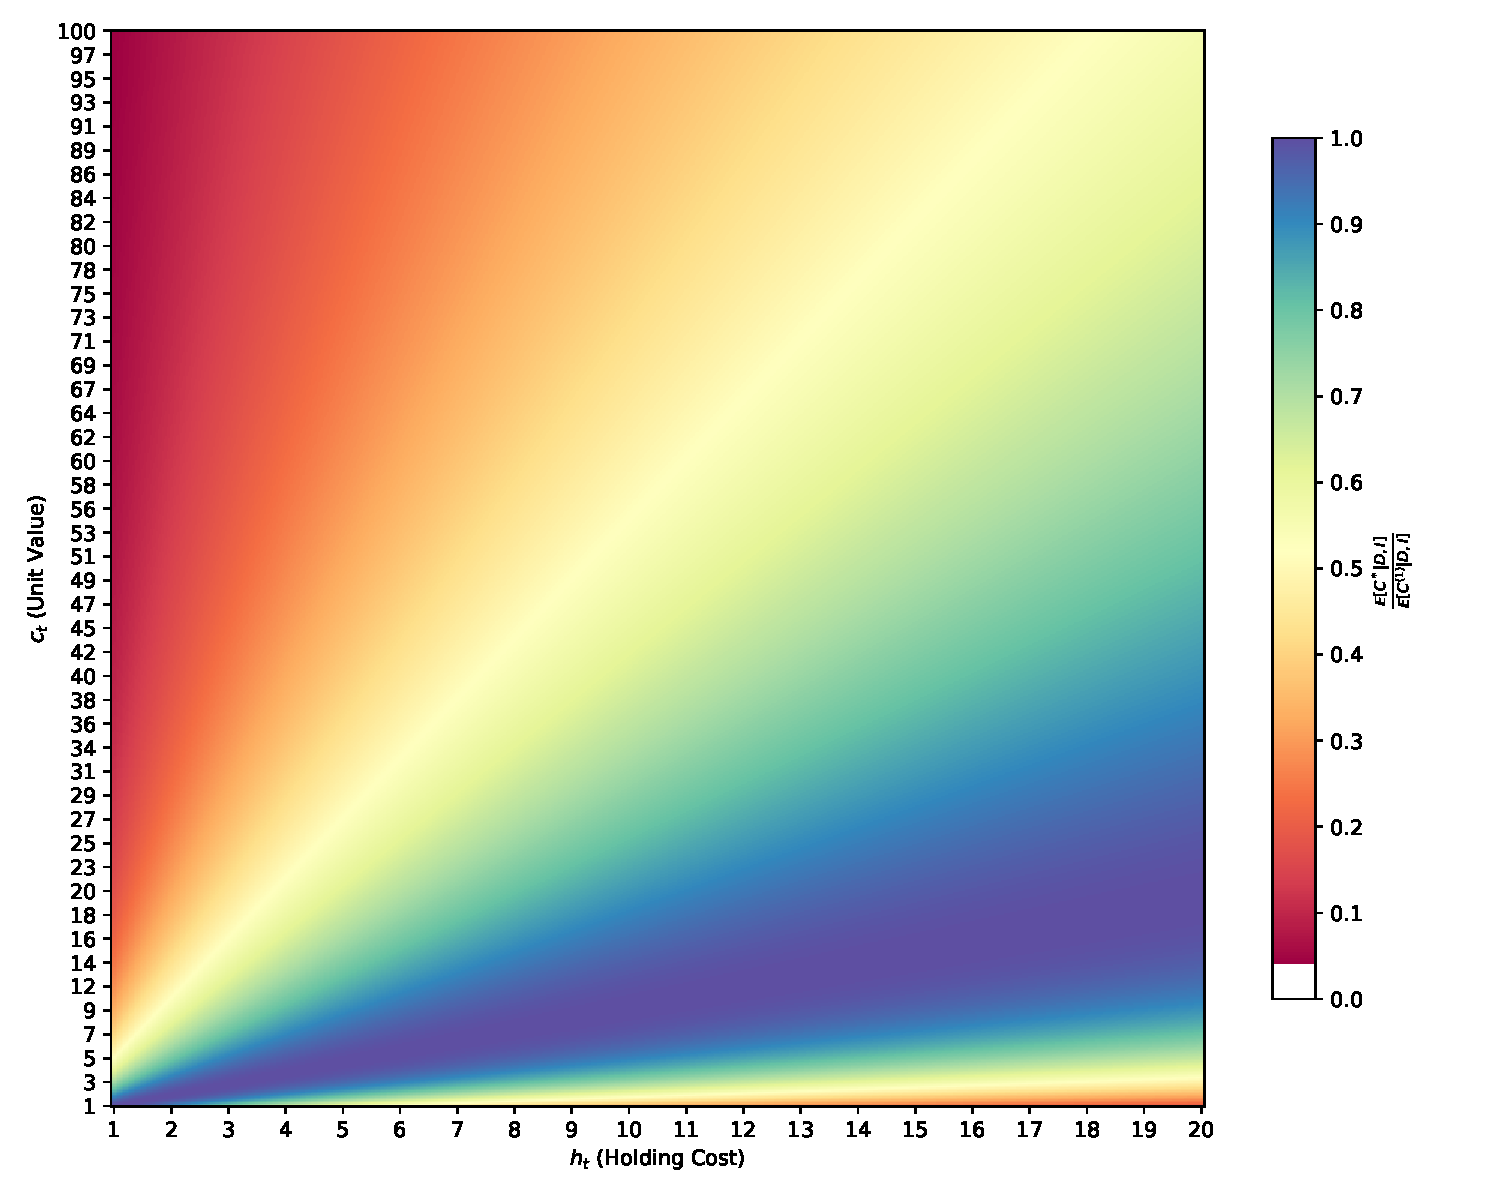
\includegraphics[width=\textwidth]{figures/analytical_per.pdf}
	\caption{Heatmap of the analytical policy efficiency ratio (equation \eqref{eq:per}).}
	\label{fig:heatmap_analytical}
\end{figure}